\documentclass[conference]{IEEEtran}
\IEEEoverridecommandlockouts
% The preceding line is only needed to identify funding in the first footnote. If that is unneeded, please comment it out.
\usepackage{cite}
\usepackage{amsmath,amssymb,amsfonts}
\usepackage{algorithmic}
\usepackage{graphicx}
\usepackage{textcomp}
\usepackage{xcolor}
\usepackage{kotex}
\usepackage{makecell}
\usepackage{float}
\usepackage{tabularx}
\usepackage{longtable}
\usepackage{multicol}
\usepackage{listings}
\usepackage{cleveref, array, booktabs, threeparttable}
\usepackage{array}
\usepackage{tabu} 
\usepackage{enumitem}
\usepackage[export]{adjustbox}
\def\BibTeX{{\rm B\kern-.05em{\sc i\kern-.025em b}\kern-.08em
    T\kern-.1667em\lower.7ex\hbox{E}\kern-.125emX}}
\begin{document}

\title{Soriham\\
{\footnotesize \textsuperscript - Leave Messages via Speaker - }
\thanks
}

\author{\IEEEauthorblockN{Jungi Kim}
\IEEEauthorblockA{\textit{Dept. of Information System} \\
\textit{Hanyang University}\\
Seoul, Republic of Korea\\
damnum3@hanyang.ac.kr}
\and
\IEEEauthorblockN{Raone Park}
\IEEEauthorblockA{\textit{Dept. of Information System} \\
\textit{Hanyang University}\\
Seoul, Republic of Korea\\
raonepark@hanyang.ac.kr}
\and
\IEEEauthorblockN{Yunseok Oh}
\IEEEauthorblockA{\textit{Dept. of Information System} \\
\textit{Hanyang University}\\
Seoul, Republic of Korea\\
grade854@hanyang.ac.kr}\\
}
\maketitle

\begin{abstract}
In the past, we left a note letter on top of the table and used something like post-it to leave messages to other people but as the devices are used often, people started to send messages to a phone. But the problem is that there are so many notifications on the phone that makes people hardly remember the messages they received. Nowadays, more and more devices that are embedded with an AI speaker are being released. So we thought what will it be if we could leave a message on the AI speaker. Soriham is a service that allows a user to leave a message to an AI speaker and reads a received message when the user wants to hear it. Users can leave a message by leaving a voice to an AI Speaker or use an application to write a text message and send it to the AI Speaker. And the AI speaker that received a message will read it when the user wants to read it. Soriham also uses an AI voice mimic system, by gathering users’ voice data. Most of the AI speakers has only limited voices to reply and communicate with the users. We thought that it will be much friendlier if the users could apply their voice data to a speaker and allow the AI speaker to mimic their voices. 
\end{abstract}

\begin{IEEEkeywords}
voice, AI speaker, children, message, communication
\end{IEEEkeywords}

\section{Introduction}

\begin{table}[ht!]
\caption{Role Assignments}
\def\arraystretch{1.24} \small
    \begin{tabular}{|p{1.8cm}|p{1.4cm}|p{4.4cm}|}
    \hline
    Roles & Name & Task description and etc. \\ \hline
    User/\par Customer&  Yunseok Oh & Even though developers and managers make a good application, if there is no feedback, it is hard to find unknown errors. He will think of ideas and specify people`s needs, and design functions and application UI. After testing the results of the development team, he will give and feedback from the consumer's point of view. \\ \hline
    
    Software \par Developer & Jungi Kim & oftware developer engages in identifying, designing, installing and testing a software system he has built.  Write codes and make sure it executes. If an error occurs, the developer modifies the code and restart the program and check the services run well. Software developer helps in maintaining and updating the program to ensure that all problems are fixed. The software developer also creates an application that allows users to do specific tasks on an application. \\ \hline
    
    Development \par manager & Raone Park & The development Manager always checks whether each member is performing appropriate tasks and performs the general task of managing the development to proceed success-fully. Developer Manager analyzes what platform will be appropriate to use and find the best one. If there is a problem on the platform, he will try to find the solutions. \\ \hline
    \end{tabular}
\end{table}

\subsection{Motivation}
Modern people live a very busy life these days. People are very busy taking care of their careers, hobbies, health, etc. To organize this busy daily life, people usually manage their schedules, write diaries, or simply write notes on their smartphones. However, even if we organize them like that, there are things we forget in our daily lives. Things such as taking out laundry in the washing machine or feeding pets are often forgotten after being immersed in other things. 

It may be simple to prevent forgetting as above. If we hear again about what we have to do or what we have to recognize, we will never forget. Setting an alarm can be a way not to forget, but we thought it would be better to hear what we should do with a familiar voice than to listen to a loud ringtone (or bell sound). And by sending a message or notification to a speaker, we could communicate with people near the AI speaker.

There are also other people who need the voice messages like a young child who don't have smartphones, old people who can't read text well, and disabled people who are uncomfortable communicating through text messages from digital devices. Voice calls are also a good means of communication, but children may not have a smartphone, and adults may not be able to communicate properly at the time they want because they do not always carry it around. And it is hard to call when we are working.

Whether we have to leave a message or listen to the message, there are situations in which we cannot do such things at the exact time we want.
In this case, if we leave a voice message on the speaker in advance, it will be less burdensome for both people who leave a message and who receive the messages. For example, before parents go their work, they can leave a message to their child to take a shower and do homework after school, or someone may leave a message he/she hasn't told the disabled at home before going out.

Voice is an important thing for humans. The voice is the very emblem of the speaker, indelibly woven into the fabric of speech. In this sense, each of our utterances of spoken language carries not only its own message but also, through accent, tone of voice and habitual voice quality it is at the same time an audible declaration of our membership of particular social regional groups, of our individual physical and psychological identity, and of our momentary mood. Voices are also one of the media through which we (successfully, most of the time) recognize other humans who are important to us—members of our family, media personalities, our friends, and enemies. Currently, most of the AI speaker has a limited voice. And the voices that are given may not be satisfied, so if we could mimic the voice of the users we will be able to recognize who is the sender of the message, and feel much friendlier.

\subsection{Research on Related Software}
There are some concepts that uses AI speaker to send a message, mimics a voice by using AI, and reads a schedule that are previously registered.

\begin{enumerate}
    \item Kakao\\
    - Kakao has released an artificial intelligence speaker called Mini Hexa. Using this speaker, there is a function of checking and sending messages using a pre-registered KakaoTalk account.
    \item Google Calender\\
    - Google Calendar is a time-management and scheduling calendar service developed by Google. Google Calendar allows users to create and edit events. Reminders can be enabled for events, with options available for type and time. It can also be connected to an AI speaker and ask the schedule that the user registered in advance.
    \item Lion Rocket\\
    - This company uses deep learning technology to output desired sentences with the voice of the person who wants to enter text. Examples of such voices include one's own voice generation and the voices of famous people such as existing celebrities and presidents. In addition, by developing these technologies, it has the technology to perfectly reproduce the way virtual characters actually speak their voices (like mouth shapes).
    \item TypeCast\\
    - The company also uses voice AI technology, which has a simpler UI and makes it easy for anyone to extract the desired voice with only text. In addition, there is a great advantage here in that even after setting the voice, the tone of the voice can be adjusted to create a more colorful feeling in the same voice. In addition, the voice created in this way can be downloaded and used as a file.
\end{enumerate}

\section{Requirements}
\subsection{Voice Message}
\begin{enumerate}
    \item Leave Messages via voice\\
    - Through AI Speaker, users can freely leave messages they want to leave. First, a user wakes up the speaker by calling the speaker's name. After that, the speaker can enter the stage of receiving messages with the user's command "I want to leave a message." The speaker asks the user, "Who is the person who leaves a message?". After the user answers who he/she is (eg. mother, husband), the speaker says, "I checked. Please tell me what message you want to leave" and then receives the user's message. After receiving all the messages, the speaker asks the user once more, "Do you have more messages to add?" and when the user answers "No," it ends, but when the answer is "Yes," it says "Okay. Tell me the message you want to leave" and then receives the user's message.
    \item Leave messages via text(application)\\
    - If there is a message that the user has failed to leave as a voice on the speaker, he/she can leave a message as text on an external application. After logging in to this application with a social account, the user can leave a message on the connected speaker when the user's account is confirmed that his account is connected to the speaker. The user can leave a message in text in the 'Leave a message' menu in the application. Messages written in text on the application are sent to the speaker and left.
    \item Check the messages left\\
    - After the user calls and wakes up the speaker, it checks first if there is a message left by someone else with the command "Is there any message left behind?". If there is no message left, the speaker will sleep with a notification saying, "There is no message left behind," and if there is a message left, the speaker will ask, "Do you want to check the message left behind?" When the user answers, "Please check the message left behind," the AI speaker reads the message left behind. If there are multiple messages left, once one message ends, the speaker once again asks the user, "Would you like to check the next message?"
\end{enumerate}

\subsection{AI Voice}
\begin{enumerate}
    \item Setting the voice of the speaker similar to user's voice\\
    As above, when the user leaves a message, the speaker asked the user 'who leaves the message'. After dividing the voice by each user, each user's voice is learned so that the speaker's voice can be finally set as the user's voice (or as similar as possible), not the existing AI voice.
\end{enumerate}
\clearpage
\subsection{Application}
There are Login, Menu, Voice Setting, and Send message contents in the application. The app receives a message that the speaker spoke on the speaker when the speaker is in Soriham mode. The message from a speaker will be shown on the application. And when the user sends a message through an application, it will be sent to a speaker and reads when the user asks. The application allows users to choose voices. When the user chooses a certain voice, the text message will be converted to it.
\begin{enumerate}
    \item Log-in\\
    - After downloading an application it will lead to a page that shows us a log-in page. It will ask the user to write down an email address and a password that is previously registered. If the user doesn't have an account, clicking the register button will lead the user to a sign-up page. And if the user has forgotten the password or an id, pressing the find id/password button, will lead the user to the recovery page.
    \item Sign-up\\
    - On the sign-up page, the user should enter a name, gender, and choose a voice that a user wants to use. If the user wants to add a new voice, the user should check the permission from the application to gather voice data.
    \item Leave a Text Message\\
    - To leave a message to an AI speaker, users should choose what speaker they want to send, write down a message and press send button. If the user wants to reserve a text message to send it at a specific time, press the reserve button and choose the specific time that the user wants.
    \item Manage sent messages\\
    - To delete the sent message, users should press a text message long time to see a small menu and choose the delete button. And if the users want to change a sent message to a reserve message, press a text message long time and choose the reserve button from a small menu, and choose the change to reserve button.
\end{enumerate}

\section{Development Environment}

\subsection{Choice of Software Development Platform}
\begin{enumerate}
    \item Platform
    \begin{itemize}
        \item Android\\
        - “Soriham” needs to be on a mobile platform for quick access and easy use. So, for our program, we have chosen the Android mobile operating system as the platform. Android is the best-selling mobile OS in the world, which has the largest mobile OS share which is about 71\%. And also, software for development on Android is widely available and it`s free.\\\\\\
        
        
        
        
    \end{itemize}
    \item Programming Language\\
    \begin{enumerate}
        \begin{figure}[h!]
            \centerline{\includegraphics[width=3cm]{img/logo/javascript.png}}
            \caption{JavaScript}
        \end{figure}
        \item JavaScript\\  
        - JavaScript is an object-based script language mainly used in web browsers along with HTML and CSS. HTML gives meaning to raw content, CSS formats the displayed content, and finally JavaScript interactive content and formatting.
        - It is an advanced multi-paradigm and supports event-based, functional, and command-type programming styles. Despite the original purpose of creating a web browser, it is now possible to build a server. JavaScript is also platform-independent. This is the main reason why we choose JavaScript. In particular, React-native is used as the front end and Node.js is used as the backend.
        \begin{figure}[h!]
        \centerline{\includegraphics[width=3cm]{img/logo/python.png}}
        \caption{Python}
        \end{figure}
        \item Python\\
        - Python is interpreted, object-oriented, and high level. The programming language Python supports modules and packages. Its interpreter and extensive standard library are available in source or binary form free of charge for all major platforms and are freely distributed.
    \end{enumerate}
    \item Development Environment
    \begin{enumerate}
        \begin{figure}[h!]
            \centerline{\includegraphics[width=3cm]{img/logo/reactnative.png}}
            \caption{ReactNative}
        \end{figure}
        \item React-Native\\
        - React Native is an open-source mobile application framework developed by Facebook. It is used to develop applications for Android, iOS, Web, and UWP, and allows developers to use React along with native platform functions.
         \begin{figure}[h!]
            \centerline{\includegraphics[width=3cm]{img/logo/tensorflow.png}}
            \caption{Tensorflow}
        \end{figure}
        \item TensorFlow\\
        - TensorFlow is an open-source library that is popular with Machine Learning. TensorFlow offers APIs that facilitate Machine Learning. The goal is to implement this AI model in using NUGU speakers.
         \begin{figure}[h!]
            \centerline{\includegraphics[width=3cm]{img/logo/NUGU.png}}
            \caption{NUGU PlayBuilder}
        \end{figure}
        \item NUGU Playbuilder\\
        - NUGU Playbuilder connects to NUGU speaker to support SK Telecom's artificial intelligence speaker NUGU various services. Whose platform first identifies the user's intention to speak through speech recognition and natural language understanding. Then, it behaves and reacts appropriately in text-to-speech. NUGU Playbuilder is a GUI-based integrated development environment that provides the necessary technology for this process.
         \begin{figure}[h!]
            \centerline{\includegraphics[width=3cm]{img/logo/google cloud.png}}
            \caption{Google Cloud}
        \end{figure}
        \item Google Cloud\\
        - Google Cloud forms the center of Google’s cloud computing platform Google Web Services, allowing users to rent virtual computers and run their own computer applications on them. We use this for backend development.
        \begin{figure}[h!]
            \centerline{\includegraphics[width=3cm]{img/logo/amazon.png}}
            \caption{Amazon}
        \end{figure}
        \item AWS\\
        - AWS (Amazon Web Services) is a comprehensive, evolving cloud computing platform provided by Amazon that includes a mixture of infrastructure as a service (IaaS), platform as a service (PaaS) and packaged software as a service (SaaS) offerings. AWS services can offer an organization tools such as compute power, database storage and content delivery services.
         \begin{figure}[h!]
            \centerline{\includegraphics[width=3cm]{img/logo/firebase.png}}
            \caption{Firebase}
        \end{figure}
        \item Firebase\\
        - Firebase is a toolset to “build, improve, and grow your app”, and the tools it gives you cover a large portion of the services that developers would normally have to build themselves, but don’t really want to build, because they’d rather be focusing on the app experience itself. This includes things like analytics, authentication, databases, configuration, file storage, push messaging, and the list goes on. The services are hosted in the cloud, and scale with little to no effort on the part of the developer.
         \begin{figure}[h!]
        \centerline{\includegraphics[width=3cm]{img/logo/figma.png}}
        \caption{Figma}
        \end{figure}
        \item Figma\\
        - Figma is a vector graphics editor and prototyping tool which is primarily web-based, with additional offline features enabled by desktop applications for macOS and Windows. The Figma Mirror companion apps for Android and iOS allow viewing Figma prototypes in real-time on mobile devices. The feature set of Figma focuses on use in user interface and user experience design, with an emphasis on real-time collaboration.
        \begin{figure}[h!]
        \centerline{\includegraphics[width=3cm]{img/logo/Github.png}}
        \caption{Git/Github}
        \end{figure}
        \item Git and Github\\
         - Git and Github offer three main functions. The first is version control. Git is a version control system that stores the timing and content of changes to the file. The second is backup. If the data is stored only on the local computer, the data will be lost and must be saved. GitHub is Git's remote repository that provides online backup. Finally, Github offers strong collaboration capabilities. When people work as a team, they can push and pull source code to remote storage to work together.\\\\
         \begin{figure}[h!]
        \centerline{\includegraphics[width=3cm]{img/logo/visual paradigm.png}}
        \caption{Visual Paradigm}
        \end{figure}
        \item Visual Paradigm\\
        - It is a UML CASE tool that supports UML2, SysML, and Business Process Modeling Notation (BPMN) of the Object Management Group (OMG). In addition to modeling support, it also provides report generation and code engineering functions, including code generation. It is possible to reverse engineer diagrams in code and provide reciprocating engineering for various programming languages.
    \end{enumerate}
\end{enumerate}

\subsection{Software in use}
There are companies that use AI speaker to send messages to a phone such as "Mini Hexa" which is from Kakao, "Giga Genie" from KT, and "Google Home" from Google. However, our "Soriham" differs from existing services in that it has the function of reading the messages that are sent from a phone. 

And there are some companies that use AI voice to read a text message such as "Lion Rocket" and "TypeCast". However, "Soriham" uses not only an AI voice that is previously registered, but it also gathers data of a voice of a user and speaks with the user's voice when enough data is stored.

\begin{enumerate}
    \item Mini Hexa\\
    - It is Kakao Enterprise's fourth smart speaker released in October 2020. As an official sequel to Kakao Mini C, it is a product that has been improved and developed in all aspects as a whole. It is equipped with "voice recognition beamforming" and "eco-cancelation" functions with six far-field microphones that are two more than the previous work, greatly improving the direction and recognition rate of whispering voices, distant voices, and loud environments. Qualcomm's smart audio 400 platform has upgraded performance, connectivity, and audio functions. It is on sale for 59,000 won as a regular price for Kakao Talk gifts.
    \item Giga Genie\\
    - It is an artificial intelligence speaker family equipped with a set-top box function that was first released by KT in January 2017. For the first time in the world, IPTV and artificial intelligence will provide a home assistant function linked to TV.It was introduced as a comment. All GiGA Genie monopolizes manufacturing in Gaon Media.
    GiGA Genie 1 and 2 were released as smart speakers and were sold separately, and existing Olleh TV subscribers can purchase/lease them without a separate agreement. Within a year of launch, the number of subscribers surpassed 500,000.
    \item Google Home\\
    - Google Nest is a smart speaker family developed by Google. The devices allow users to speak voice commands to interact with the service through Google Assistant, the company's virtual assistant. Both in-house and third-party services are integrated so that you can listen to music, control the playback of videos or photos, or receive news updates entirely by voice. The first device, Google Home, was released in the United States in November 2016, and has since been released worldwide since 2017.
    \item Lion Rocket \& Type Cast \\
    - Lion Rocket and a TypeCast is an artificial intelligence voice actor service that allows users to use specific voices to read a text. Anyone can easily download a voice that seems to have been recorded by a professional performer just by entering a script and simple editing.
\end{enumerate}

\subsection{Task Distribution}

\begin{table}[htbp]
\begin{center}
\caption{Task Distribution}
\begin{tabular}{|l|l|}
\hline
Name        & Task description          \\ \hline
Yunseok Oh  & Backend                   \\ \hline
Jungi Kim   & Frontend, Play Builder    \\ \hline
Raone Park  & Frontend, Play Builder    \\ \hline
\end{tabular}
\end{center}
\end{table}
Task Distribution is shown in Table 2. Each member has his own main role, but since we do not know much about programming, we ask each other, share our thoughts and ideas to improve our project, and proceeds.

\section{Specifications}

\subsection{AI Speaker}
\begin{enumerate}
    \item Voice Message
    \begin{enumerate}
        \item Leave a message using voice\\
        - The speaker receives the message when the user asks the speaker to receive a voice message.
        
        - When the user asks to start a message mode "소리함 켜줘", the speaker will ask the name of the sender "작성자의 이름이 무엇인가요?" the time that the message will arrive, "언제 메세지를 남겨드릴까요?" the message that user wants to send, "남기실 메세지를 말씀해 주세요" and confirmation message."000님이 몇시에 말씀하신 메세지가 ~ 로 남길까요?"
        
        - If the user says "응 남겨줘", the speaker will send a message but if the user says "틀렸어 다시해줘", "시간 몇시로 바꿔줘", "이름을 000로 바꿔줘", "메세지 바꿔줘" and the speaker will change the specific part that the user asked to do and asked the confirmation message again.
        \item Message left using text in app\\
        - In the application, the user could go to the messenger part, write down the messages that the user wants to send, and it will be sent to the speaker.
        
        - The speaker receives the text message that the user sent on the application.
        \item Adjust the received messages\\
        - If the Speaker receives a message, the speaker will give a ringtone as a signal.
        
        - If there are unread messages in the speaker, the led of the speaker will blink.
        
        - User could check the messages by asking a speaker to read them.
        
        - Users could check how many messages there are by asking "메세지 몇개 있어?" and the speaker will reply, "현재 몇개의 메세지가 있습니다."
        
        - User could delete the received messages by asking "메세지 삭제해줘". And the speaker will reply "삭제되었습니다".
    \end{enumerate}
    
    \item Voice
    \begin{enumerate}
        \item Basic Voice\\
        - There are several voices that are given, and the users could choose a voice that they want to send a message. Users can choose the voice depending on the mood, emotion, and feelings that the user currently has
        
        - By the voice that the user chose, the speaker will read the message.
        \item AI Voice
        \begin{itemize}
        \item Voice machine learning\\
        - By following the steps, the user could record their voice to TTS.
        
        - If the record is successfully done, the voice of the user will be a part of the voice option. 
        
        - If the user chooses a voice to a voice that the user recorded, the user will be able to ask the speaker to read text messages using the user's voice.
        \end{itemize}
    \end{enumerate}
\end{enumerate}

\subsection{Application}
\begin{enumerate}
    \begin{figure}[ht!]
    \centerline{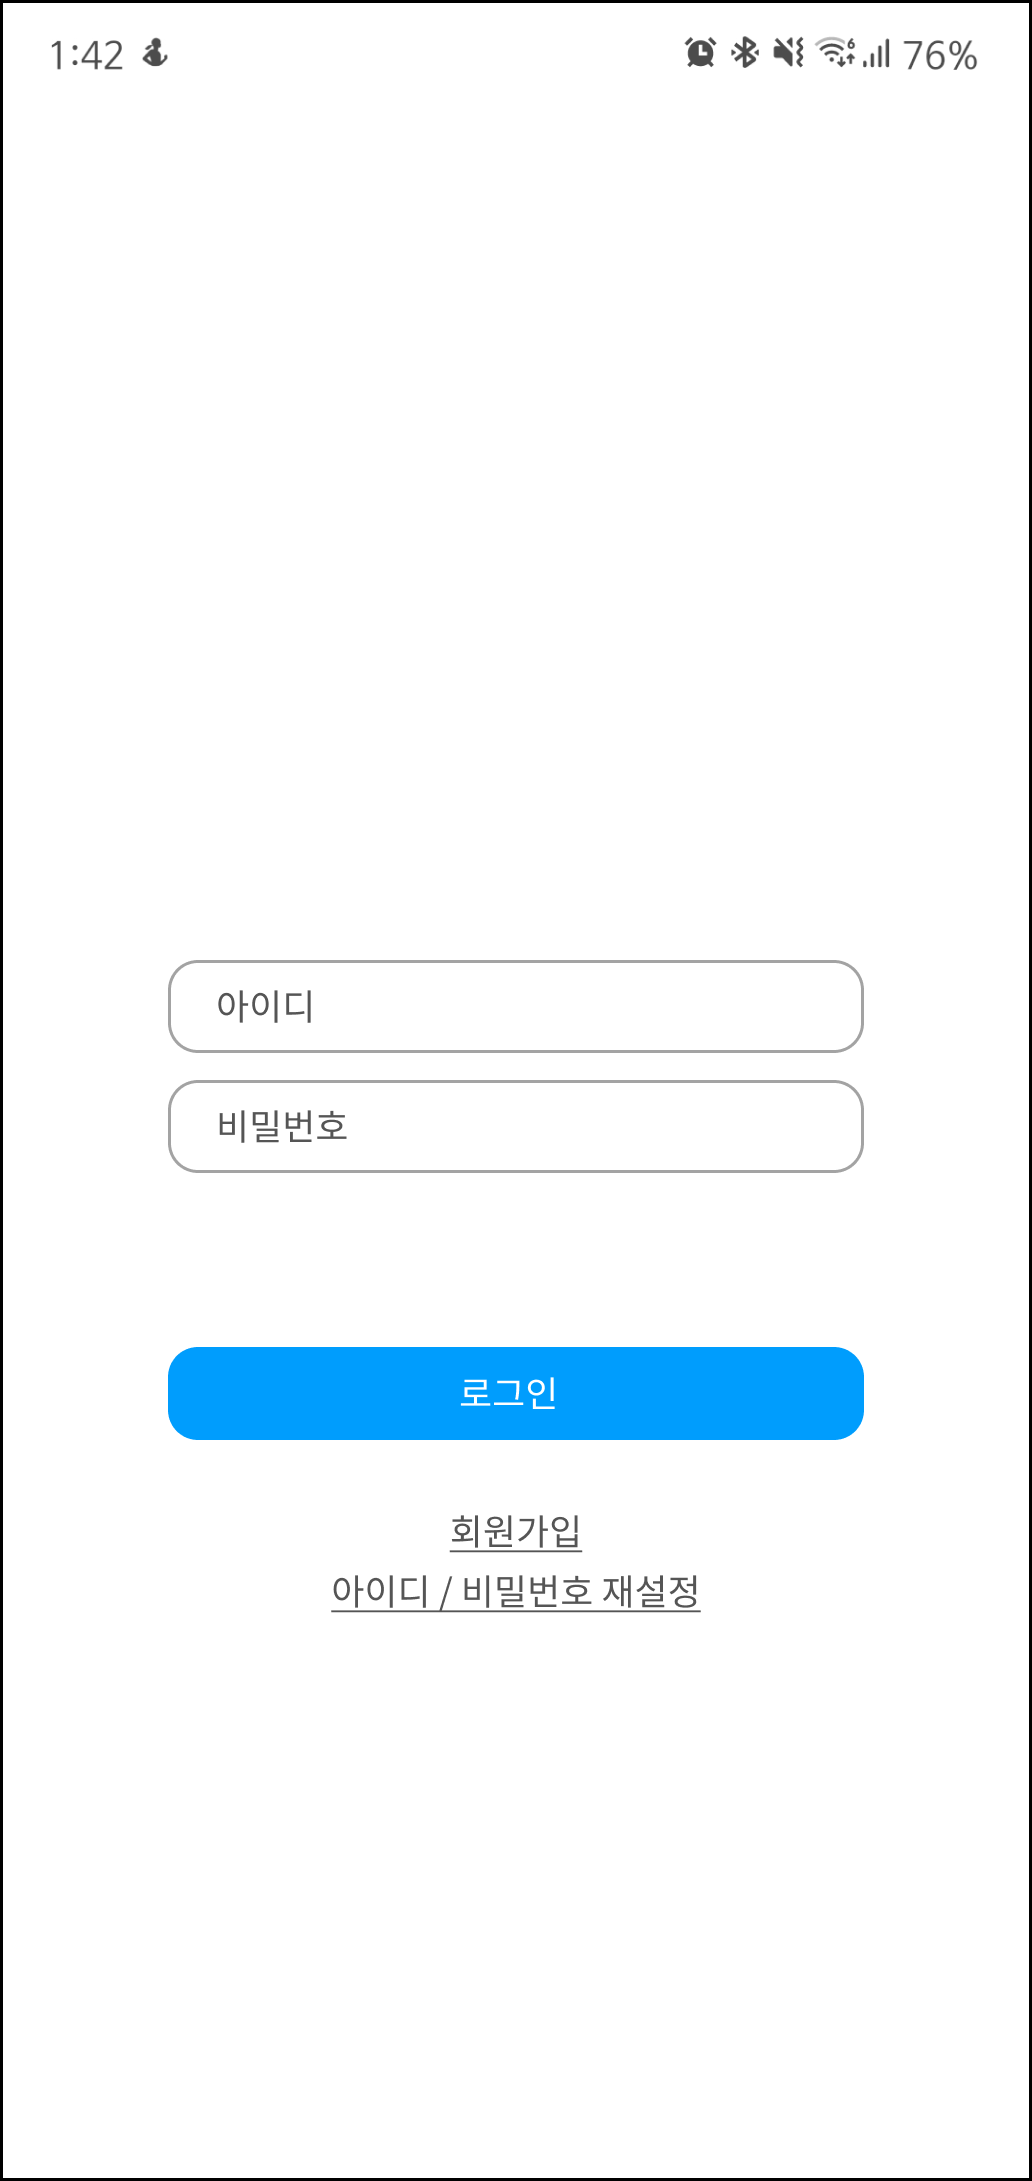
\includegraphics[width=4cm]{img/Login.png}}
    \caption{Login}
    \end{figure}  
    \item Login [Fig.1]\\
    - The user could login through typing a ID that is registered in SKT NUGU Smart Home.
    
    - After the user succeeds in logging in, the user goes to the main page where 'send messages' and 'voice setting' menu are existing.
    \begin{figure}[ht!]
    \centerline{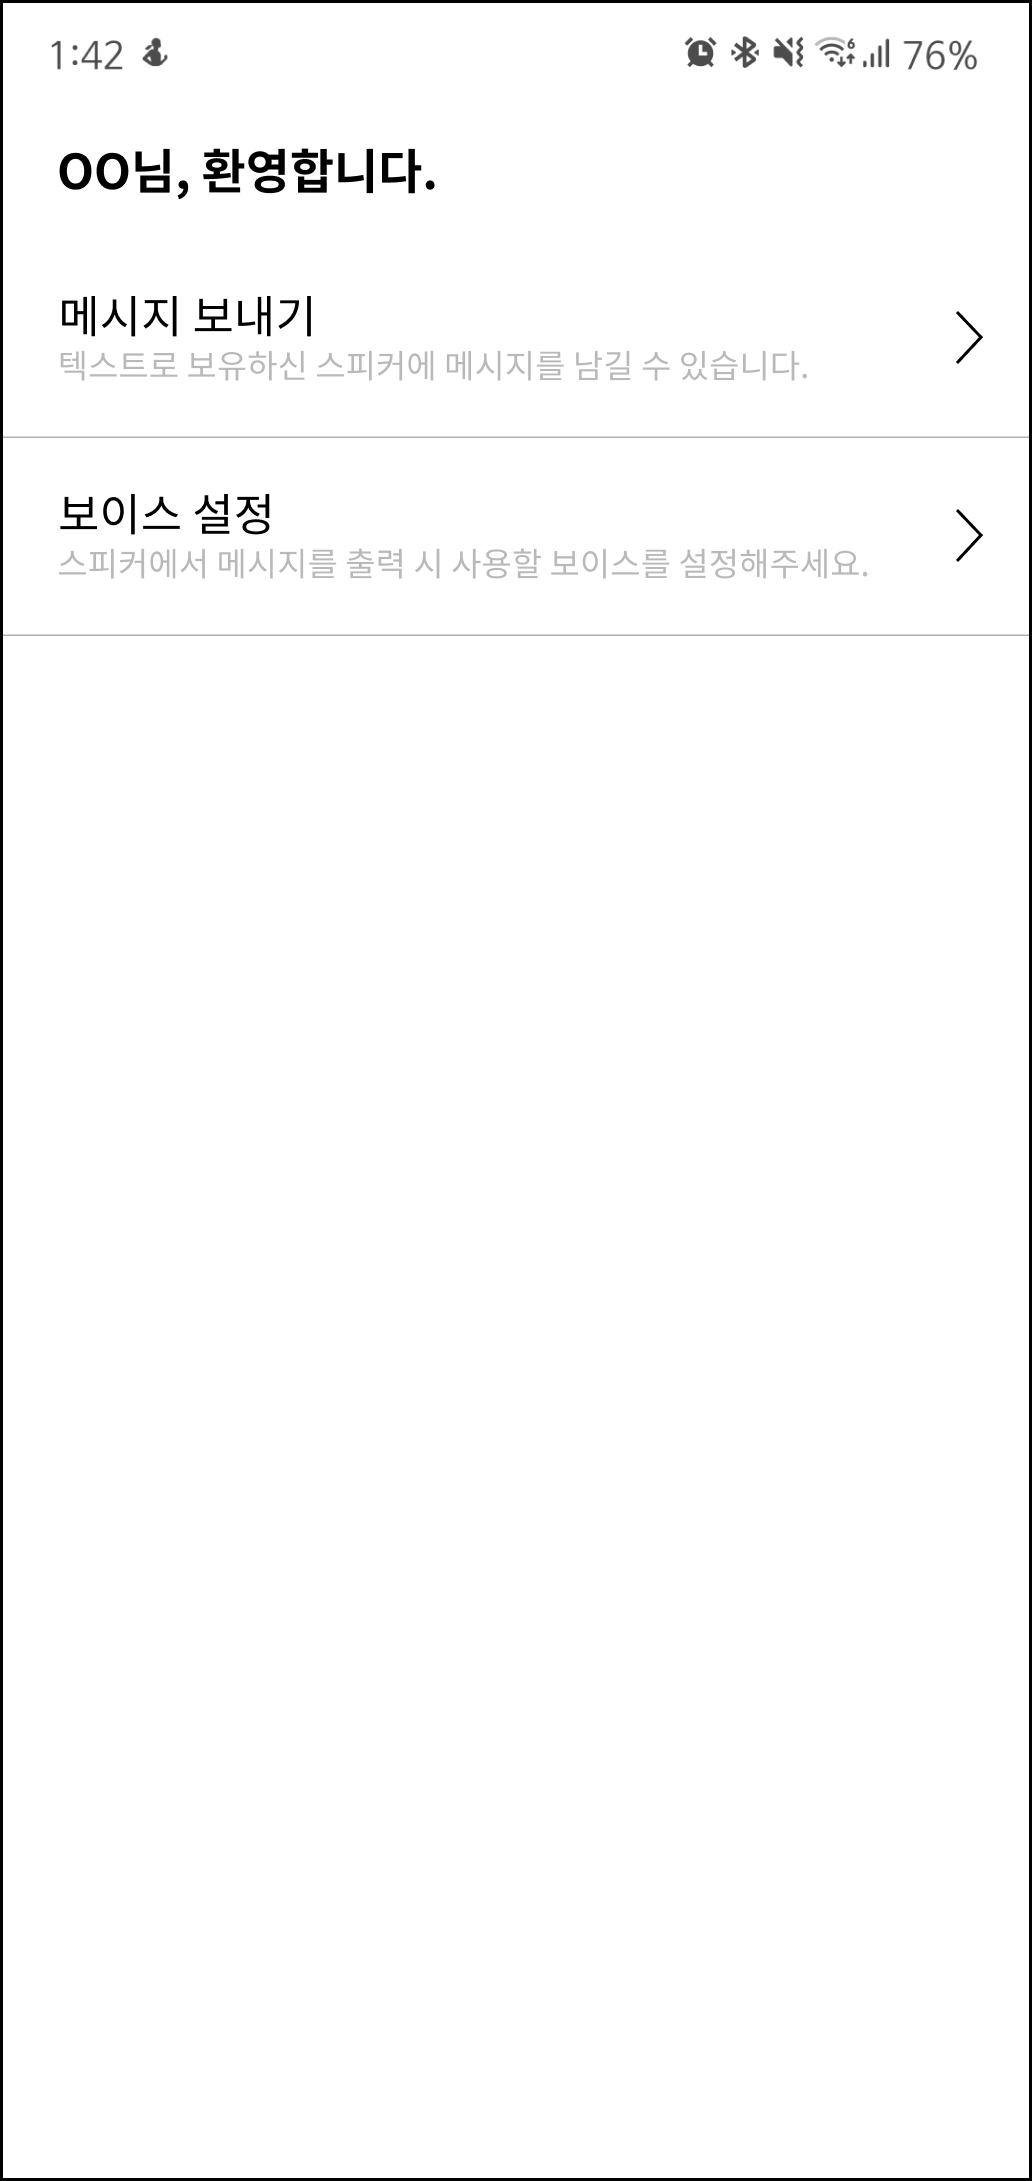
\includegraphics[width=4cm]{img/Main.png}}
    \caption{Main}
    \end{figure}  
    \item Main Page [Fig.2]\\
    - There are two menus, to send a message and a Voice setting that a user wants to send.
    
    - When the user chooses the first option which is to send a message, it will lead the user to Send Message page.
    
    - When the user chooses the option which is voice setting, it will lead the user to the Voice Setting page.
    \begin{figure}[ht!]
    \centerline{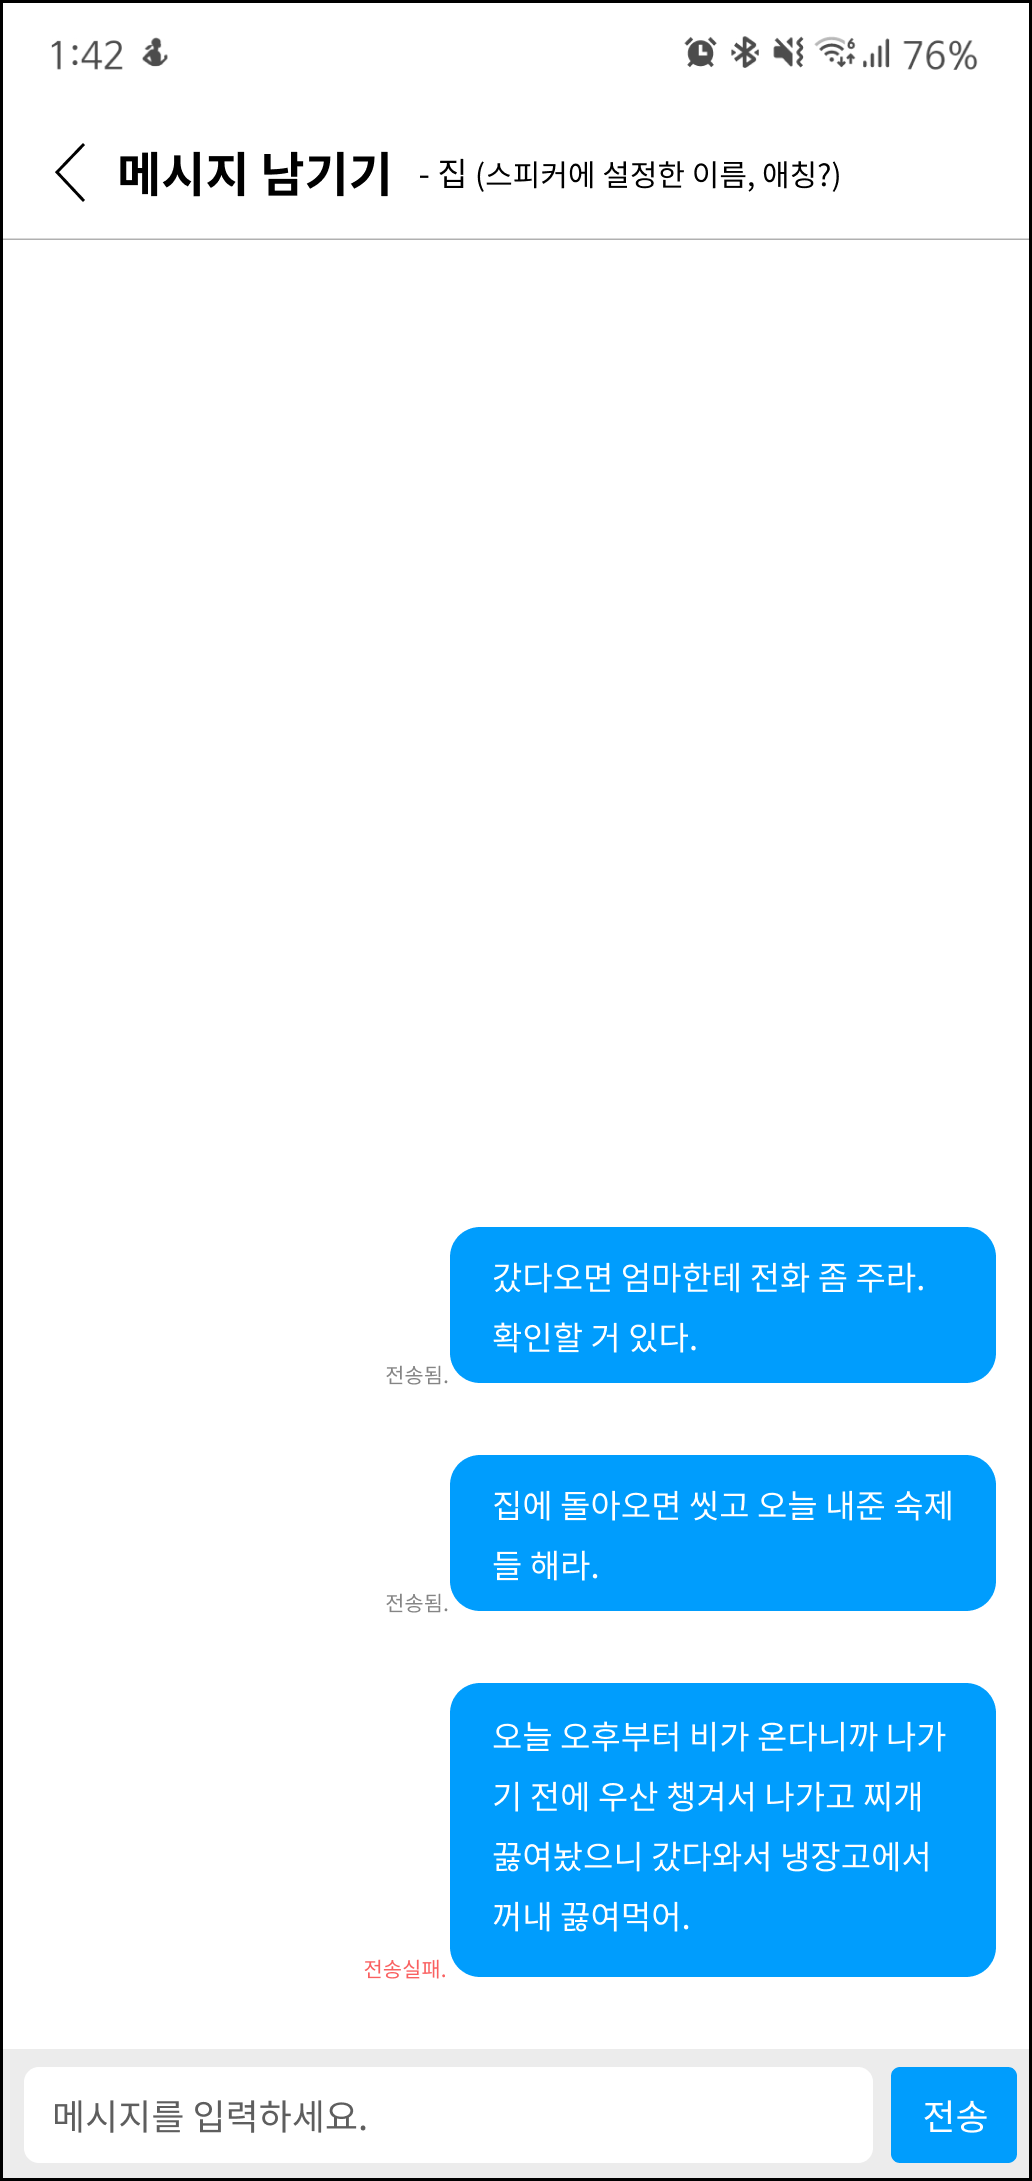
\includegraphics[width=4cm]{img/Message.png}}
    \caption{Send Messages}
    \end{figure}  
    \item Send Message [Fig.3]\\
    - The user could type a message and send it by pressing the send button.
    
    - The length of the message cannot exceed 140 characters in English and 70 characters in Korean.
    
    - If the message entered in text was well sent to the speaker, the mark '전송됨' appears next to the message sent. But if not, '전송실패' appears. The user can resent the failed message using copy and paste.
    
    - By pressing a sent message for 3 seconds, the delete button will pop out.
    
    - If someone else hears a message sent in text through a speaker, the "전송됨" mark will be changed to a "읽음" mark. Messages changed to "읽음" marks cannot be deleted.
    
    - On the top left, there is a button that lets the user go back to the Main page.
    \begin{figure}[ht!]
    \centerline{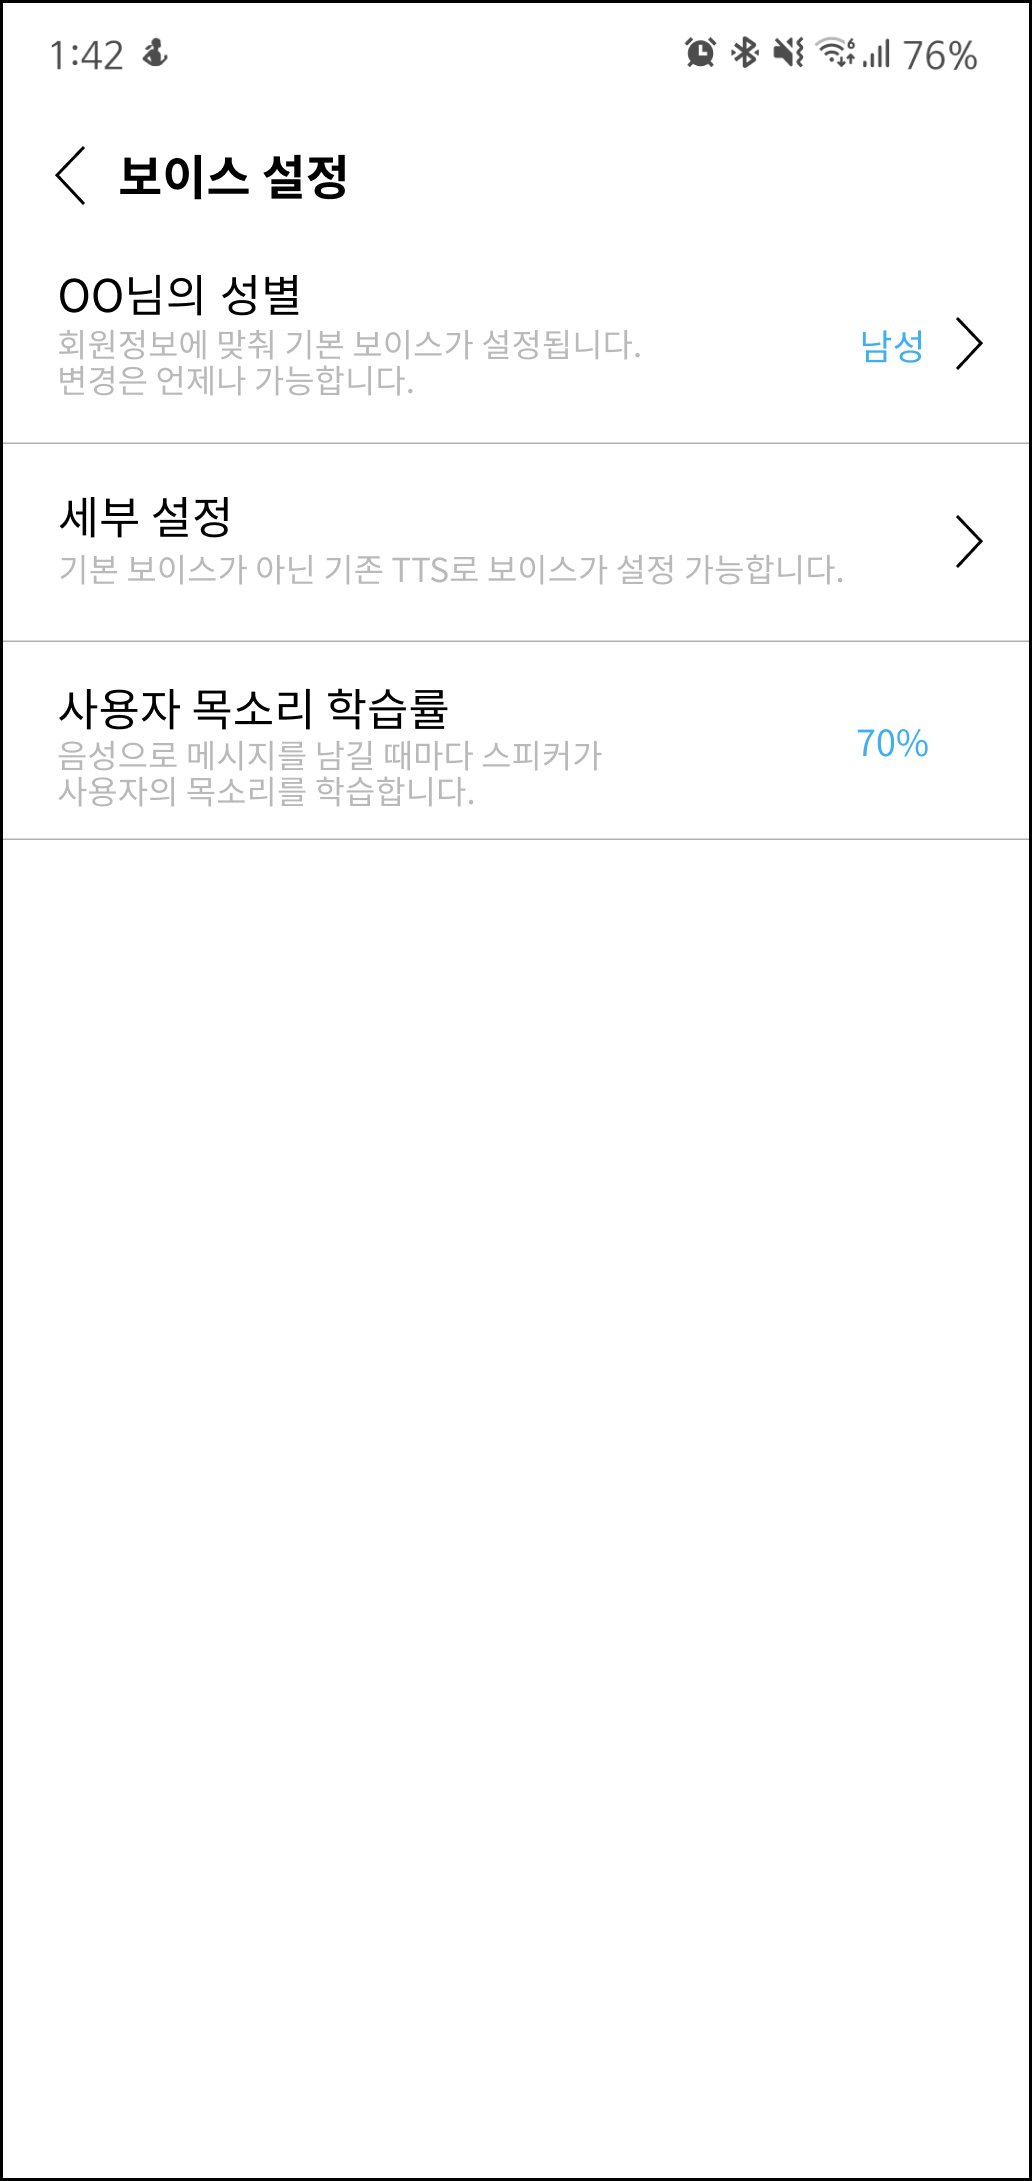
\includegraphics[width=4cm]{img/Setting - Voice.png}}
    \caption{Voice Setting}
    \end{figure} 
    \item Voice Setting [Fig.4]
    \begin{enumerate}
        \item Gender\\
        - The default gender setting follows the information entered when the user registered.
        
        - The user can change between the two (male/female) anytime the user wants.
        \begin{figure}[ht!]
        \centerline{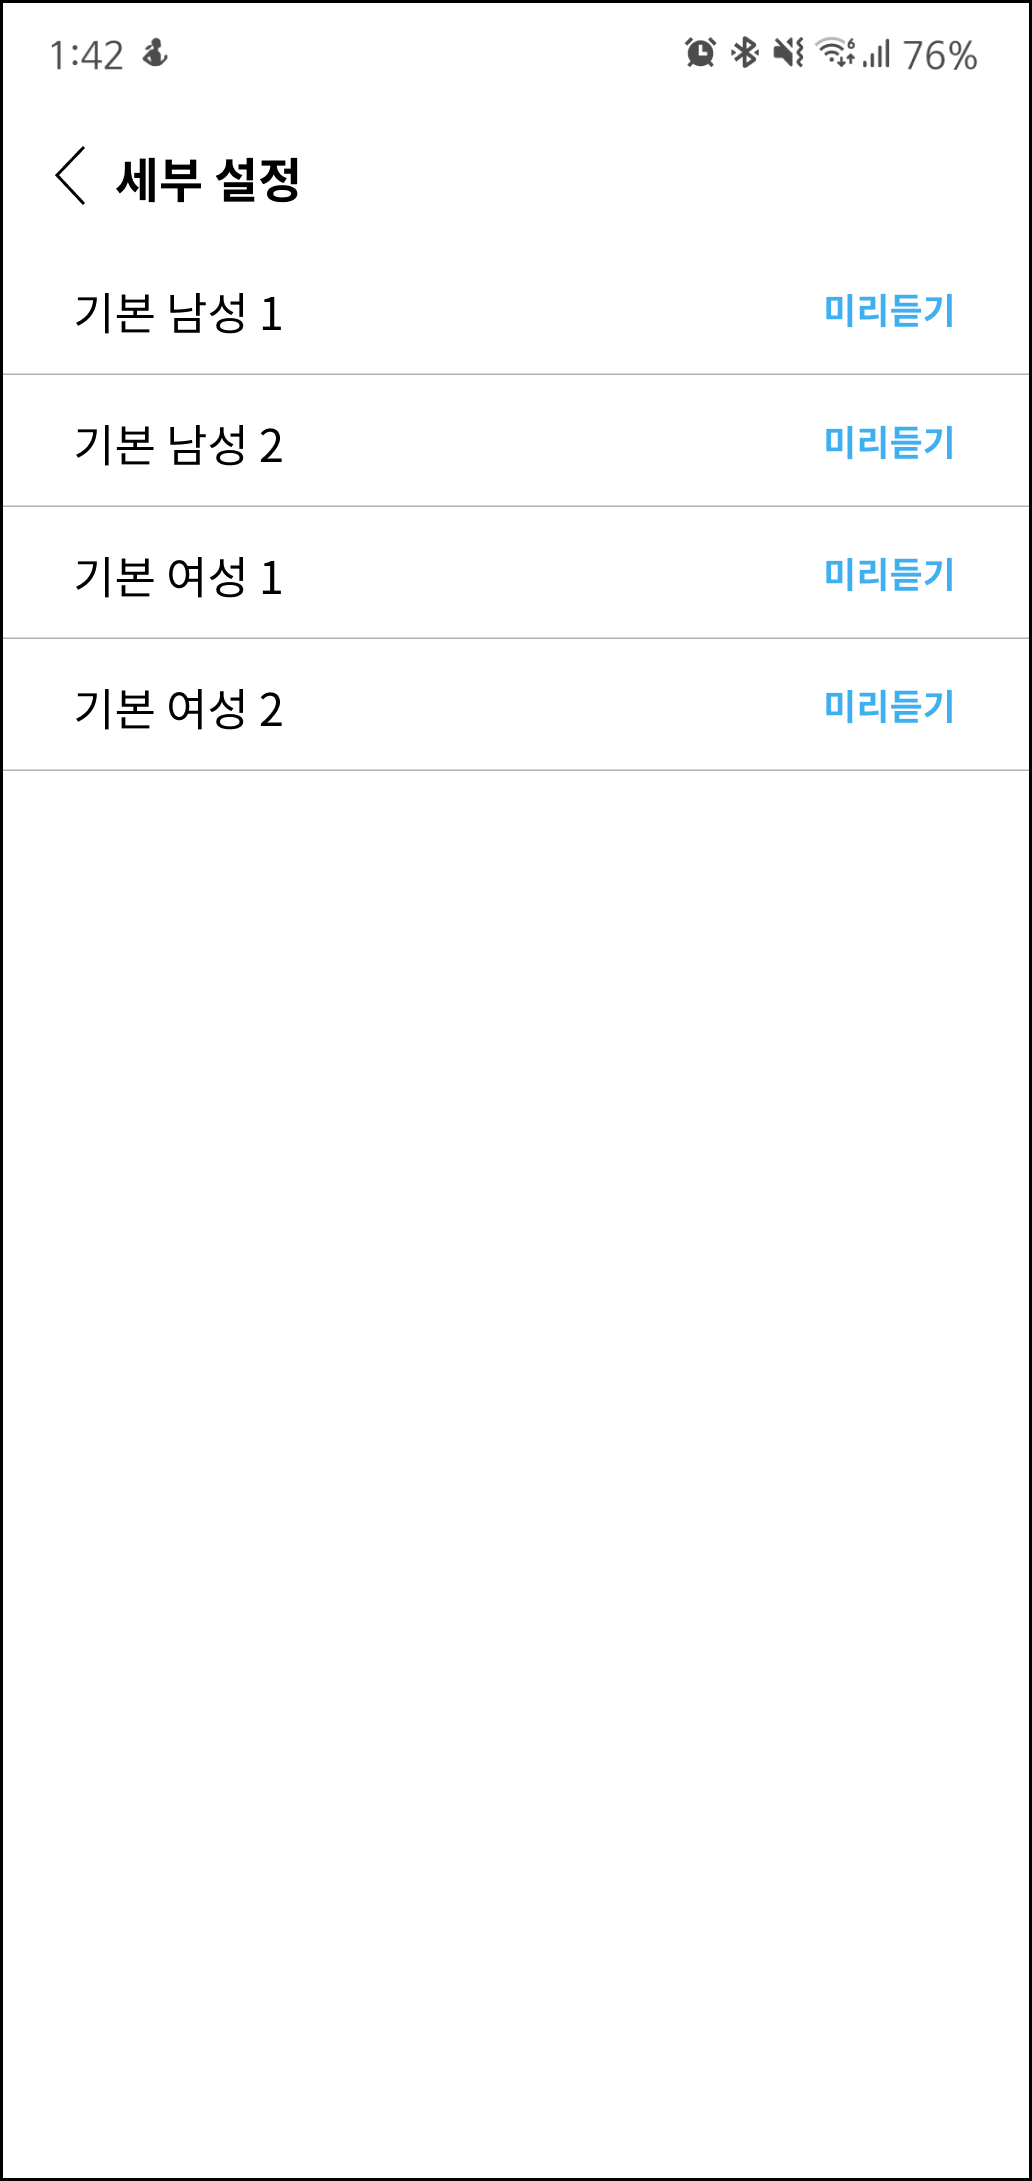
\includegraphics[width=4cm]{img/Setting - Voice - Detail.png}}
        \caption{Voice Detail Setting}
        \end{figure} 
        \item Voice Detail [Fig.5]\\
        - Users can set their voice with the existing TTS, not the user's own voice.
        
        - The user can listen to the sample voice by pressing the '미리듣기' button for each TTS before choosing a voice.
        
        - If enough data is gathered for AI voice, users could choose an option to use AI voice.
    \end{enumerate}
\end{enumerate}

\section{Architecture Design \& Implementation}
\subsection{Overall Architecture}
\begin{figure*}[htb!]
    \centering
    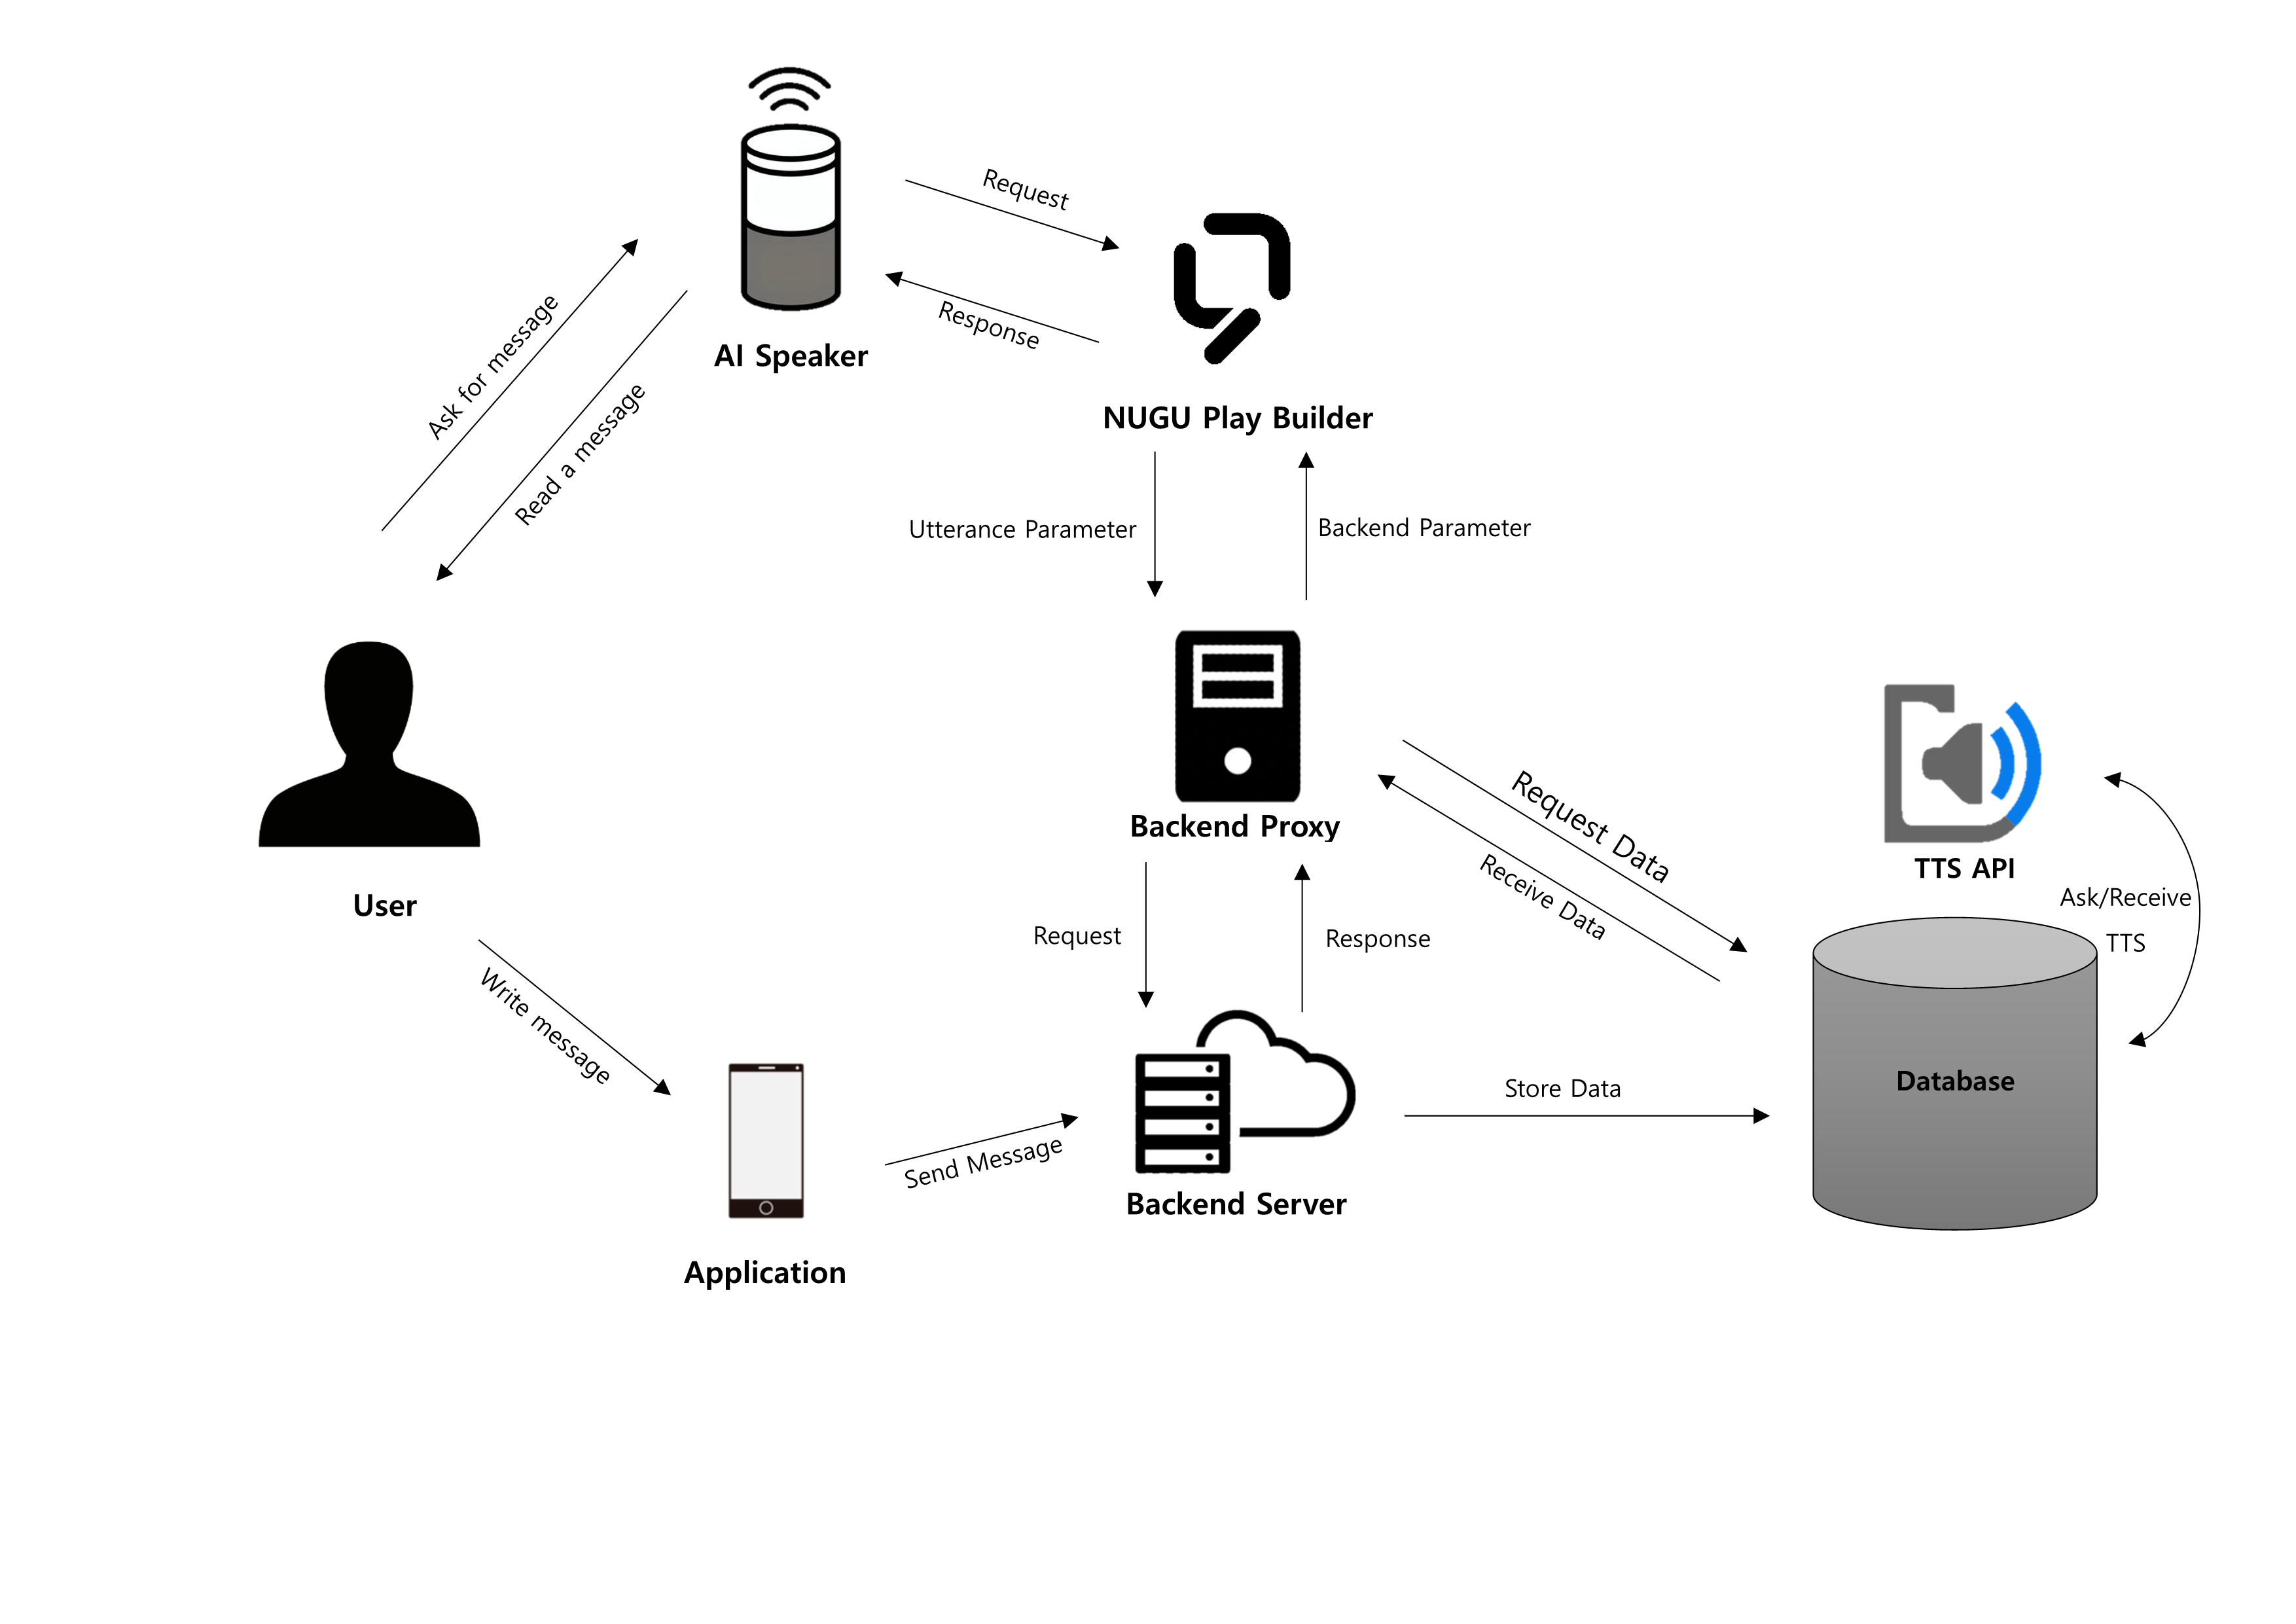
\includegraphics[height=10cm]{img/Overall Architecture.png}
    \caption{Overall Architecture}
\end{figure*}
- Soriham is divided into two main modules: the frontend and the backend (see Figure). The frontend is compatible with its own git and is available on Android or IOS devices. Send a request to the backend server to get data when you are connected to the Internet using this application(program).

- The backend server has two endpoints (who, message). The server performs the necessary tasks based on what AI Speaker requests. If a user uses a request to “save”, the backend server identifies who it is with a parameter called who, determines which message it is, and stores it in the database. For example, when a father saves the message "Eat dinner" on a server, “who” is the father, and “message” is "Eat dinner" and then saves it.
In addition, two endpoints (who, message) are also used when using the message import function. When a user requests to retrieve a message, the backend server identifies who came with a parameter called “who”, requests the stored message to the TTS server, converts it into the person's TTS, and responds to the backend server.

- When response from the TTS server arrives on the backend server, the server responds to the data back to the AI Speaker and processes it in a way that is played by the AI Speaker.
\subsection{Directory Organization}
\begin{enumerate}
    \begin{table}[ht!]
    \centering
    \caption{Client Directory}
    \label{tab:server-dircetory-table}
        \begin{tabular}{|l|l|l|}
        \hline
        \textbf{Directory}        & \textbf{File name}                                                              & \textbf{Module}                                              \\ \hline
        front-end/                & App.js                                                                          & React                                                        \\ \hline
        front-end/config          & firebase.js                                                                     & \begin{tabular}[c]{@{}l@{}}firestore\\ firebase\end{tabular} \\ \hline
        front-end/screens/main    & \begin{tabular}[c]{@{}l@{}}Login.js\\ Main.js\end{tabular}                      & \begin{tabular}[c]{@{}l@{}}React\\ Native\end{tabular}       \\ \hline
        front-end/screens/message & Chat.js                                                                         & \begin{tabular}[c]{@{}l@{}}React\\ Native\end{tabular}       \\ \hline
        front-end/screens/voice   & \begin{tabular}[c]{@{}l@{}}VoiceSetting.js\\ VoiceSettingDetail.js\end{tabular} & \begin{tabular}[c]{@{}l@{}}React\\ Native\end{tabular}       \\ \hline
        \end{tabular}
    \end{table}
    \item Client Directory
    \begin{enumerate}
        \item App.js\\
        - App.js is a bridge of the application. It connects all of the page of an application and allows to display it.
        \item firebase.js\\
        - firebase.js is used to import the function of the firebase. By writing down the firebaseconfiguration such as apiKey, authDomain, projectId and others, we could connect it to our project that is in firestore database.
        \item Login.js\\
        - Login.js lead user to write down their id \& password. User should click '회원가입' if the user doesn't have an id.
        \item Main.js\\
        - Main.js is shown when the user login the application. It lead user to choose what page to go. User could go to the Chat page, VoiceSetting page by clicking a button.
        \item VoiceSetting.js\\
        - VoiceSetting.js is shown when the user press '보이스 설정'. User could change the gender, go to the VoiceSettingDetails, and see the value of User's voice learning rate.
        \item VoiceSettingDetails.js\\
        - VoiceSetting Details.js is shown when the user press '세부설정'. Users could choose what kind of AI voice to send a TTS message. If the user press '미리듣기', the sample voice will be played.\\
    \end{enumerate}
    \begin{table}[ht!]
    \centering
    \caption{Backend Proxy Directory}
    \label{tab:backend-proxy-directory-table}
        \begin{tabular}{|l|l|l|}
        \hline
        \textbf{Directory}        & \textbf{File name} & \textbf{Module}                                                              \\ \hline
        back-end-proxy/mySoriham/ & index.js           & \begin{tabular}[c]{@{}l@{}}AWS Lambda\\ Amazon - \\ API Gateway\end{tabular} \\ \hline
        \end{tabular}
    \end{table}
    \item Backend Proxy Directory
    \begin{enumerate}
        \item index.js\\
        - 'Play' exports appropriate responses or performs actions based on the analysis of the user's speech. If the information needed for this response needs to be imported from an external server, it must be requested through REST API, and because the sound must be played in the '소리함', the definition of the Directive command must also be handled by the backend proxy.
        
        - In this file, refer to the specified format (Backend proxy API standard) shown in the NUGU Developer Guide, we can find the Action Name and parameters of the Request. After that, appropriate Response is also defined according to the action name and parameters.
    \end{enumerate}
    \begin{table}[ht!]
    \caption{Machine Learning Directory}
    \label{tab:machine-learning-dircetory-table}
    \centering
        \begin{tabular}{|l|l|l|}
        \hline
        \textbf{Directory}          & \textbf{File name}                                                                                       & \textbf{Module}                                             \\ \hline
        machine-learning/           & \begin{tabular}[c]{@{}l@{}}infer-v2.ipynb\\ train-glowtts-v2.ipynb\\ train-hifigan-v2.ipynb\end{tabular} & \begin{tabular}[c]{@{}l@{}}Glow-TTS\\ HiFi-GAN\end{tabular} \\ \hline
        machine-learning/data       & filelists.zip                                                                                            &                                                             \\ \hline
        machine-learning/glowtts-v2 & \begin{tabular}[c]{@{}l@{}}glowtts-v2-'Training complete \\ data generation date'\end{tabular}           & Glow-TTS                                                    \\ \hline
        machine-learning/hifigan-v2 & \begin{tabular}[c]{@{}l@{}}hifigan-v2-'\\ Training complete \\ data generation date'\end{tabular}        & HiFi-GAN                                                    \\ \hline
        \end{tabular}
    \end{table}
    \item Machine Learning Directory
    \begin{enumerate}
        \item infer-v2.ipynb\\
        - This file is a file that creates a completed TTS model by synthesizing the learned glow-TTS model and the hifigan-TTS model.
        \item train-glowtts-v2.ipynb\\
        - This file is a file that learns the glow-TTS model using the data set of the user's voice. Through this learning, you can derive results with a feeling similar to the user's tone and pitch. However, when conducting only this learning, a sound that seems to be mixed with machine sounds is extracted.
        \item train-hifigan-v2.ipynb\\
        - This file is a file that learns the Hifigan-TTS model using the database of the user's voice. This learning makes the tone of the result similar to the actual speaker. Through this, only Glow-TTS learning is synthesized with the model to create a real model.
        \item filelists.zip\\
        - This file contains the data set required for machine learning. The actual user records about 1200 sentences and creates a dataset.
        \item glowtts-v2-'Trained data'\\
        - It contains a learning model file of the user who has completed the glow-TTS learning. You can listen to the test file of the learned model through test\_audio in this file. In addition, voice synthesis will proceed later using the best\_model.pth.tar file.
        \item hifigan-v2-'Trained data'\\
        - It contains the learning model file of the user who has completed the hifigan-TTS learning. Use the best\_model\_000000.pth.tar file to synthesize the voice later.
    \end{enumerate}
\end{enumerate}

\subsection{Modules}
\begin{enumerate}
    \item React\\
    - React is a declarative, efficient, and flexible JavaScript library for building user interfaces. It lets developers compose complex UIs from small and isolated pieces of code called “components”.
    \item React Native\\
    - React Native combines the best parts of native development with React, a best-in-class JavaScript library for building user interfaces. React primitives render to native platform UI, meaning our app uses the same native platform APIs other apps do. Soriham application is oriented for both Android iOS. We used react-native with mixture of JavaScript and XML for our development IDE. 
    \item Firebase\\
    - Firebase is a development platform known originally for its realtime database that’s still at its core a multi-node, key-value database optimized for synchronizing data, often between user machines or smartphones and centralized storage in the cloud. It’s designed to make life easier for developers by handling much of the pushing and pulling of data. 
    \item AWS Lambda\\
    - Lambda is a compute service that lets us run code without provisioning or managing servers. With Lambda, we can run code for virtually any type of application or backend service. All we need to do is supply our code in one of the languages that Lambda supports. We used lambda for backend proxy servers that communicate with speaker.
    \item Amazon API Gateway\\
    - Amazon API Gateway is an AWS service for creating, publishing, maintaining, monitoring, and securing REST, HTTP, and WebSocket APIs at any scale. API developers can create APIs that access AWS or other web services. We used Amazon API Gateway to handle POST request from speaker.
    \item Glow-TTS\\
    - The user records a certain amount of sentence files through the microphone to produce base data. Machine learning is conducted based on the produced recording file. Through Glow-TTS, the overall voice tone of the user is determined.
    \item HiFi-GAN\\
    -  We used HiFi-GAN to create a model that is closer to the user’s actual voice. As the time of machine learning increases, it gets closer and closer to the user’s actual voice. 
    \item TTS (Text-to-Speech) \& STT (Speech-to-Text)\\
    - Speech synthesis is the artificial production of human speech. Computer systems used for this purpose are called voice computers or voice synthesizers and can be implemented in software or hardware products. It allows Soriham to converts plain language text into speech. The text-to-speech system (or engine) consists of two parts: a front end and a back end. There are two main tasks at the front end. 
    
    - First, convert raw text containing symbols such as numbers and abbreviations equally to written words. In the first part, speech transcription is assigned to each word, and text is divided into rhyme units such as phrases, clauses, and sentences. Phonics and rhyme information together constitute symbolic language expressions output by the front end. The backend, often referred to as a synthesizer, converts symbolic language expressions into sound. In a particular system, this part includes the calculation of the target rhyme (pitch contour, phoneme duration), and is imposed on the output voice.
    
    - Speech recognition develops methodologies and techniques for computers to recognize speech language and translate it into text. The system we use requires 'training' in which individual speakers read text or isolated vocabulary into the system. This system analyzes a person's specific voice and uses it to recognize that person's tone, thereby increasing accuracy. 
\end{enumerate}

\section{Use Cases}

\subsection{User Case 1: Leave Messages Using Voice}
\begin{figure}[ht!]
    \centerline{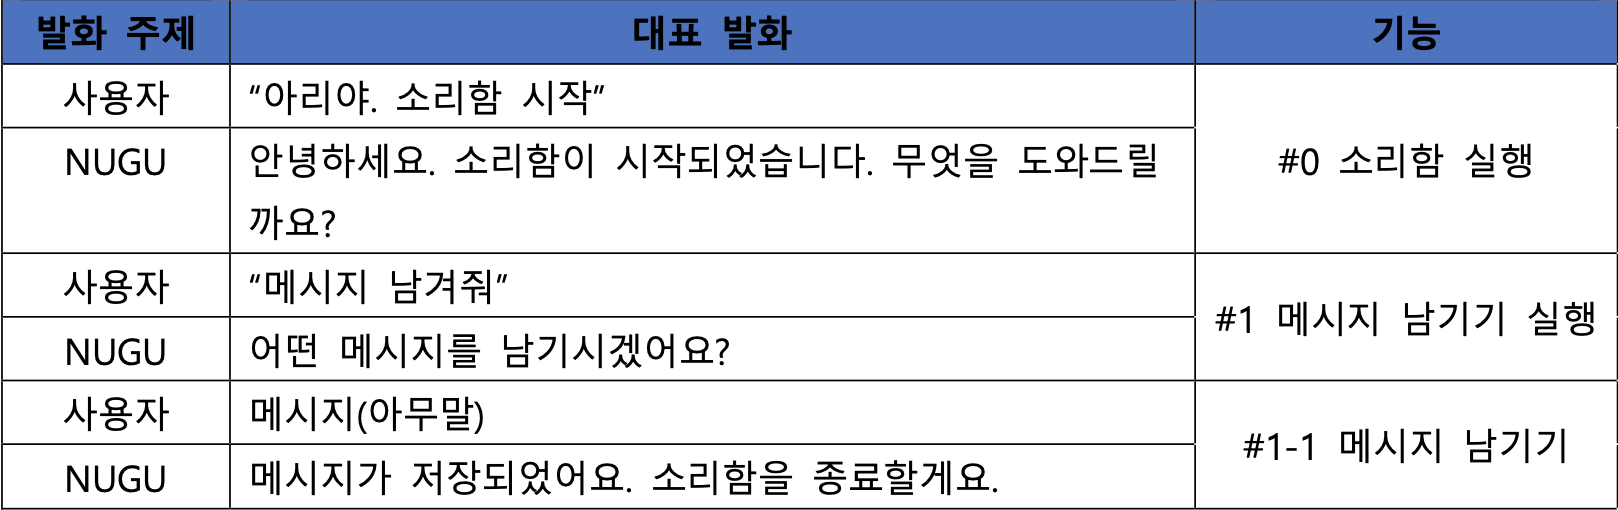
\includegraphics[width=9cm]{img/usecase 1.png}}
    \caption{User Case 1}
\end{figure}
Users can leave messages using speakers at any time they want. After the user wakes up the speaker first, the user reveals his intention by saying, "I want to leave a message." Then, the speaker grasps the intention and takes 'SoundRecordAction'. When the user leaves a message he or she wants to leave, the voice turns into text(Speech-to-Text) and moves on to the server. The text is changed to the user's voice learned through the learning model and turns into the voice (Text-to-Speech). The voice file is stored in cloud storage.
\subsection{User Case 2: Leave Messages Using Text in App}
Users can also leave messages not only using voice, but also text. If you write down the message you want to leave on the application as text and press the send button, the text will be delivered to the learning model. Text is changed to the user's voice through a learning model and stored as a voice file(it can be 'mp3' or 'm3u8').
\subsection{User Case 3: Playing Messages Left Before}
\begin{figure}[ht!]
    \centerline{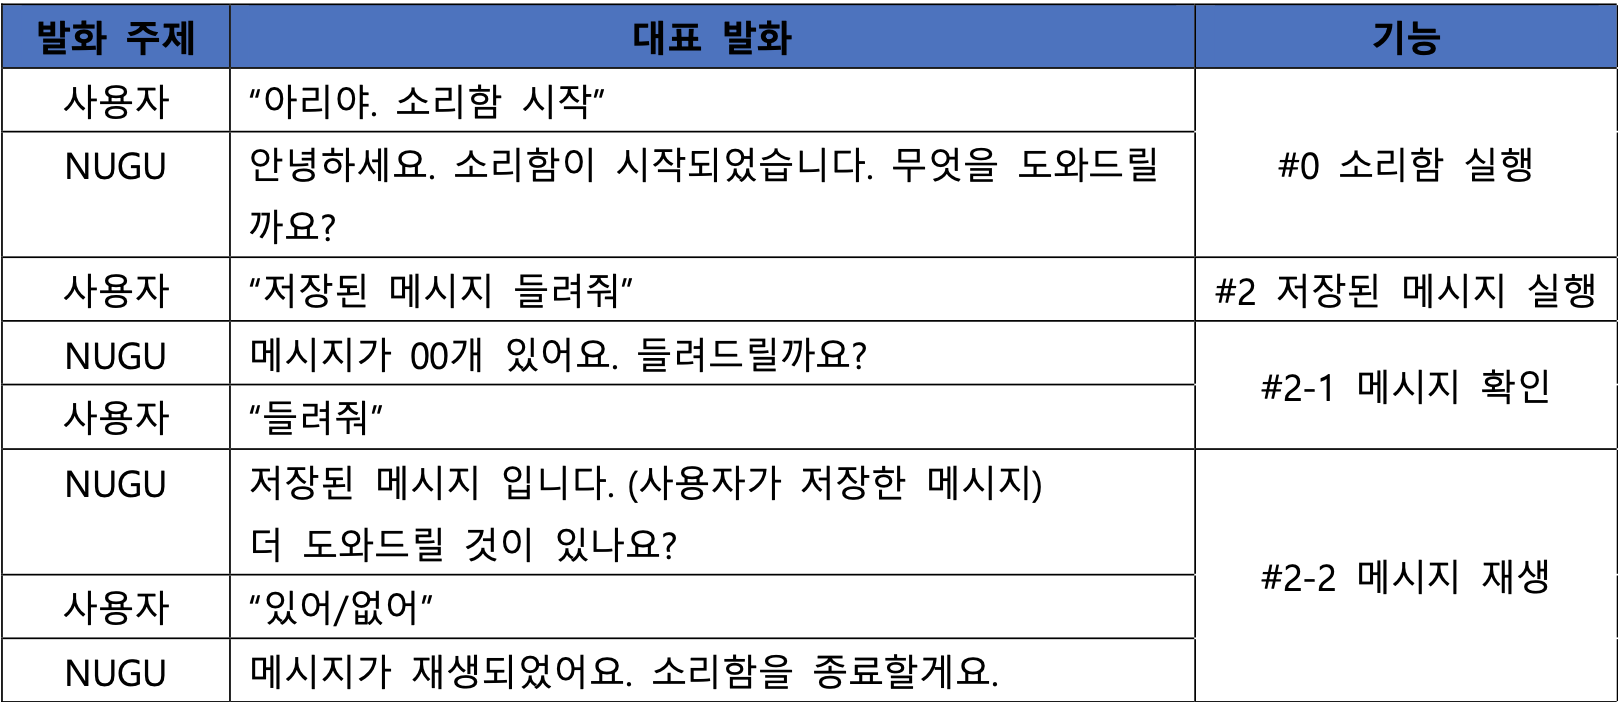
\includegraphics[width=9cm]{img/usecase 3.png}}
    \caption{User Case 3}
\end{figure}
The user can wake up the speaker at any time to check the previously left message. After the user wakes up the speaker, he reveals his intention to "play the message." Then, the speaker understands the intention and takes 'SoundPlayAction'. The URL of the message left before in the storage is retrieved and played using the speaker's audio directive function.

\begin{thebibliography}{00}
\bibitem{b1} https://www.ncbi.nlm.nih.gov/pmc/articles/PMC3361774/.
\end{thebibliography}
\vspace{12pt}

\end{document}
